\errorcontextlines 10000
\documentclass[a4paper,14pt]{memoir}
\usepackage{etoolbox}
\usepackage{multicol}

% set up fonts
\usepackage{fontspec}
\setsansfont{Titillium-Regular}
\setmainfont{Titillium-Regular}
\setromanfont{FSSinclair-Medium}

% smaller margins
\usepackage[margin=1.2cm]{geometry}

% drawing packages
\usepackage{tikz}
\usetikzlibrary{shapes}
\usetikzlibrary{decorations.text}
\usepackage{pgfplots}
\pgfplotsset{
  compat = newest,
  tick label style = {font=\sffamily},
  every axis label = {font=\sffamily},
  legend style = {font=\sffamily},
  label style = {font=\sffamily}
}

% custom colours
\definecolor{adaYellow}{RGB}{245,225,52}
\definecolor{adaPurple}{RGB}{149,96,159}
\definecolor{adaGreen}{RGB}{161,200,84}
\definecolor{adaCoral}{RGB}{236,98,113}
\definecolor{adaBlue}{RGB}{108,184,231}
\definecolor{adaOrange}{RGB}{246,131,82}

\definecolor{adaBlack}{RGB}{9,20,8}
\definecolor{adaGrey}{RGB}{134,136,140}
\definecolor{adaLightGrey}{RGB}{211,212,211}
\definecolor{adaWhite}{RGB}{255,255,255}

\definecolor{clr1}{RGB}{149,96,159}
\definecolor{clr2}{RGB}{161,200,84}
\definecolor{clr3}{RGB}{236,98,113}
\definecolor{clr4}{RGB}{108,184,231}
\definecolor{clr5}{RGB}{246,131,82}

% Declare layers
\pgfdeclarelayer{background}
\pgfsetlayers{background,main}

\setlength{\columnsep}{3em}
\begin{document}
% no page numbers
\pagestyle{empty}
% title
\begin{center}
    {\rmfamily\uppercase{
        {\large \VAR{name}}\\
        January 2020}}
\tikz[remember picture,overlay,shift=(current page.north east)] \node[inner sep=0pt] at (-2,-2) {\includegraphics[height=2cm]{NCDS.jpg}};
\end{center}
\begin{multicols}{2}
% Attendance bar chart
\noindent\makebox[\columnwidth]{\rmfamily\uppercase{Attendance}\hrulefill}
\vskip \bigskipamount
\begin{center}
\begin{tikzpicture}[scale=0.8]
\begin{axis}[
  axis y line*=right,
  axis x line*=bottom,
  symbolic x coords={Autumn 1,Autumn 2, Spring 1, Spring 2, Summer 1, Summer 2},
  xtick ={Autumn 1,Autumn 2, Spring 1, Spring 2, Summer 1, Summer 2},
  x tick label style={rotate=90,anchor=east},
  ymin = 70,
  ymax = 100,
  ytick = {70,80,90,100},
  yticklabels = {70,80,90,100},
  xticklabels = {Autumn 1,Autumn 2},
  xmin = Autumn 1,
  xmax = Summer 2,
  grid=major,
  clip=false,
  ]
  \addplot[adaGreen,line width=5pt,dashed] coordinates {(Autumn 1, 93) (Summer 2, 93)};
  \addplot[ybar, fill=adaPurple] coordinates {(Autumn 1, \VAR{attendance.aut1}) (Autumn 2,\VAR{attendance.aut2})};
\end{axis}
\end{tikzpicture}
\end{center}
\vskip \bigskipamount
% The values circle
\noindent\makebox[\columnwidth]{\rmfamily\uppercase{Values}\hrulefill}
\vskip \bigskipamount
\begin{center}
\begin{tikzpicture}[scale=0.4]
	\foreach[count=\v] \value in {Curiosity,Creativity,Collaboration,Rigour,Resilience} {
    	\draw[white,postaction={decorate,decoration={text along path, text align=center,text={|\small\sffamily|\value}}}] (72*\v:5.5) to [bend left=36] (72*\v-72:5.5);
        \draw (72*\v:5) -- (72*\v:0);
    }
    \foreach[count=\v] \value in {\VAR{values.Curiosity},\VAR{values.Creativity},\VAR{values.Collaboration},\VAR{values.Rigour},\VAR{values.Resilience}} {
        \foreach \ring in {1,...,5} {
            \draw[clr\v] (72*\v:\ring) arc (72*\v:72*\v-72:\ring);
        }
        \filldraw[fill=clr\v] (0,0) -- (72*\v:\value) arc (72*\v:72*\v-72:\value) -- (0,0);
}
\end{tikzpicture}
\end{center}
\end{multicols}
\vskip \bigskipamount
\noindent\makebox[\textwidth]{\rmfamily\uppercase{Progress}\hrulefill}
\vskip \bigskipamount
%% if subjects|length == 2 or subjects|length == 4
\begin{multicols}{2}
%% elif subjects|length == 3
\begin{multicols}{3}
%% endif
%% for subject in subjects
% Target graph
\begin{center}
\begin{tikzpicture}[scale=0.8, baseline=(current axis.south)]
\begin{axis}[
    axis y line*=right,
    axis x line*=bottom,
    symbolic x coords={\VAR{subject.ap1name},Target},
    symbolic y coords = "0",{\VAR{subject.scale}},
    scaled y ticks=false,
    xtick ={\VAR{subject.ap1name},Target},
    x tick label style={rotate=90,anchor=east},
    ymin = \VAR{subject.min},
    ymax = \VAR{subject.max},
    ytick = {\VAR{subject.ticks}},
    yticklabels = {\VAR{subject.labels}},
    xticklabels = {\VAR{subject.ap1name},Target},
    grid=major,
    clip=false,
    ]
    % title
    \node[align=left,font=\rmfamily, yshift=1em] (title) 
    at (current bounding box.north)
    {\sffamily{\VAR{subject.name}}};
	\addplot[adaGreen,line width=5pt,dashed] coordinates {(\VAR{subject.ap1name},\VAR{subject.target}) (Target,\VAR{subject.target})};
	\addplot[ybar, fill=adaGreen] coordinates {(Target,\VAR{subject.target})};
	\addplot[ybar, fill=adaPurple] coordinates {(\VAR{subject.ap1name},\VAR{subject.ap1grade})};
\end{axis}
\end{tikzpicture}
\end{center}
%% endfor
%% if subjects|length > 1
\end{multicols}
%% endif
%% if subjects|length > 3
\clearpage
%% endif
\vskip \bigskipamount
\noindent\makebox[\textwidth]{\rmfamily\uppercase{Actions}\hrulefill}
\vskip \bigskipamount
\begin{multicols}{2}
\noindent
\begin{minipage}{\columnwidth}
\noindent{\rmfamily\uppercase{Professional}} {\sffamily \VAR{professional}}
\end{minipage}
\begin{minipage}{\columnwidth}
\noindent{\rmfamily\uppercase{Academic}} {\sffamily \VAR{academic}}
\end{minipage}
\end{multicols}
\clearpage
\noindent\makebox[\textwidth]{\rmfamily\uppercase{FAQ}\hrulefill}
{\sffamily This report is intended to start conversations between students, staff and home. Rather than present overwhelming detail, we've tried to keep text to a minimum. The presentation may be new to you though, so don't hesitate to ask if anything is unclear.}\\
\noindent{\rmfamily\uppercase{Attendance}}\\
\noindent{\sffamily What does the green dashed line mean?}\\
\indent {\sffamily The dashed green line represents attendance of 93\% which is our minimum expectation.}\\
\noindent{\rmfamily\uppercase{Values}}\\
\noindent{\sffamily How is the values circle calculated?}\\
\indent {\sffamily When staff award \emph{kudos points} to students, we record which of our values the student has shown.
The size of the slice is calculated from the number of points awarded by staff over the course of the term. For example, a student who received no kudos points for curiosity, one for creativity, a few for collaboration, about ten for rigour, and even more for resilience, would have a values circle like this:}\\
\begin{center}
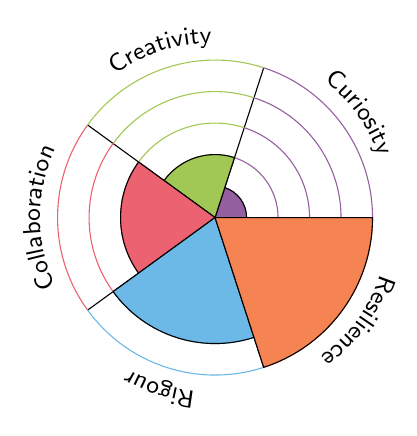
\begin{tikzpicture}[scale=0.4]
	\foreach[count=\v] \value in {Curiosity,Creativity,Collaboration,Rigour,Resilience} {
    	\draw[white,postaction={decorate,decoration={text along path, text align=center,text={|\small\sffamily|\value}}}] (72*\v:5.5) to [bend left=36] (72*\v-72:5.5);
        \draw (72*\v:5) -- (72*\v:0);
    }
    \foreach[count=\v] \value in {1,2,3,4,5} {
        \foreach \ring in {1,...,5} {
            \draw[clr\v] (72*\v:\ring) arc (72*\v:72*\v-72:\ring);
        }
        \filldraw[fill=clr\v] (0,0) -- (72*\v:\value) arc (72*\v:72*\v-72:\value) -- (0,0);
}
\end{tikzpicture}
\end{center}
\noindent{\sffamily These accumulate over the two years. So this example student can safely focus on curiosity, without worrying that their resilience sector will go down!}\\
\noindent{\rmfamily\uppercase{Targets}}\\
\noindent{\sffamily Where do the target grades come from?}\\
\indent {\sffamily These are targets that students have set for themselves to represent their ambitions for a subject.}\\
\noindent{\sffamily What do the purple bars represent?}\\
\indent{\sffamily This will vary from subject to subject. For A Levels, they will be grades from internal assessments. For Computing, they will be a recent judgment based on all the coursework and assessments completed so far.}\\
\noindent{\rmfamily\uppercase{Actions}}\\
\noindent{\sffamily Where do the actions come from?}\\
\indent {\sffamily Students have identified one professional and one academic action as part of a self-evaluation process. These should be concrete steps that they can take to improve.}\\
\end{document}